


\documentclass{article}[12pt]
\usepackage{fullpage,graphicx, setspace, latexsym, cite,amsmath,amssymb,color,subfigure}
%\usepackage{epstopdf}
%\DeclareGraphicsExtensions{.pdf,.eps,.png,.jpg,.mps} 
\usepackage{amssymb} %maths
\usepackage{amsmath} %maths
\usepackage{amsthm}

\bibliographystyle{unsrt}

\newtheorem{theorem}{Theorem}
\newtheorem{prop}{Proposition}
\newtheorem{corollary}{Corollary}
\newtheorem{lemma}{Lemma}
\newtheorem{defn}{Definition}
\newtheorem{ex}{Example}
\usepackage{float}

\def\R{\mathbb{R}}
\def\Eps{\mathcal{E}}
\def\E{\mathbb{E}}
\def\V{\mathbb{V}}
\def\F{\mathcal{F}}
\def\G{\mathcal{G}}
\def\H{\mathcal{H}}
\def\S{\mathcal{S}}
\def\P{\mathbb{P}}
\def\1{\mathbf{1}}
\def\n{\nappa}
\def\h{\mathbf{w}}
\def\v{\mathbf{v}}
\def\x{\mathbf{x}}
\def\X{\mathcal{X}}
\def\Y{\mathcal{Y}}
\def\eps{\epsilon}
\def\y{\mathbf{y}}
\def\e{\mathbf{e}}
\newcommand{\norm}[1]{\left|\left|#1\right|\right|}
\DeclareMathOperator*{\argmin}{arg\,min}
\DeclareMathOperator*{\argmax}{arg\,max}

\newcommand{\lecture}[4]{
   \pagestyle{myheadings}
   \thispagestyle{plain}
   \newpage
   % \setcounter{lecnum}{#1}
   \setcounter{page}{1}
   \setlength{\headsep}{10mm}
   \noindent
   \begin{center}
   \framebox{
      \vbox{\vspace{2mm}
    \hbox to 6.28in { {\bf ESE 680-004: Learning and Control
   \hfill Fall 2019} }
       \vspace{4mm}
       \hbox to 6.28in { {\Large \hfill Lecture #1: #2  \hfill} }
       \vspace{2mm}
       \hbox to 6.28in { {\it Lecturer: #3 \hfill Scribes: #4} }
      \vspace{2mm}}
   }
   \end{center}
   \markboth{Lecture #1: #2}{Lecture #1: #2}

   \noindent{\bf Disclaimer}: {\it These notes have not been subjected to the
   usual scrutiny reserved for formal publications. }
   \vspace*{4mm}
}

%notation

\def \E{\mathbb E}
\def \P{\mathbb P}
\def \R{\mathbb R}
\def \A{\cal A}

\begin{document}

\lecture{7}{A Whirlwind Tour of Robust Control}{Nikolai Matni}{Christopher Hsu}

\section{Model Based Reinforcement Learning and Control}
What do I have to do in order to control a system in which I do not know if my model is exactly true? There is uncertainty inherent to the output of the algorithm. With finite data how do we quantify this uncertainty. This will be a quick but wide overview of robust control.

\begin{figure} [H]
    \centering
    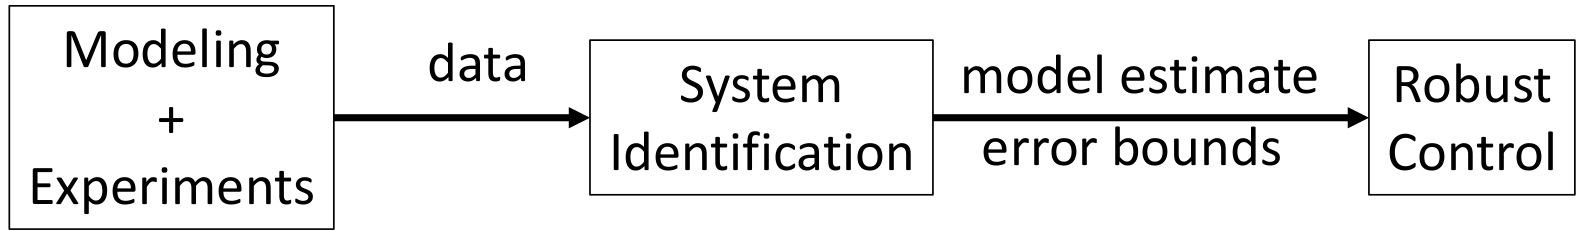
\includegraphics[scale=.2]{figures/pipeline.png}
    \caption{Learning and Control Pipeline}
    \label{fif:pipeline}
\end{figure}

To put this into perspective, previously we looked at system identification with model estimates and error bounds to be put into a robust controller. It was proved that the errors bounds could be held with high probability. We will look to test those bounds adversarially in order to do robust control. \\
    With enough experiments N can we prove with probability 1-$\delta$ that we can synthesize a robust controller that is provably near optimal and stabilizing with a relative performance bound given by:
    \begin{align*}
        \frac{\hat{J}- J_*}{j_*} &\leq C \text{(robustness, excitability)}
        \sqrt{\frac{(d+p)log(\frac{1}{\delta})}{N}}
    \end{align*}
Where d is the number of states and p is the number of inputs. Excitability is the 1 over the minimum singular value of the controllability grammian. So how can we combine this uncertainty in our model with robust control?

\section{Generalized Plant}
Let's introduce the plant, which is a generalized linear dynamical system with two outputs. 
    \begin{figure} [H]
        \centering
        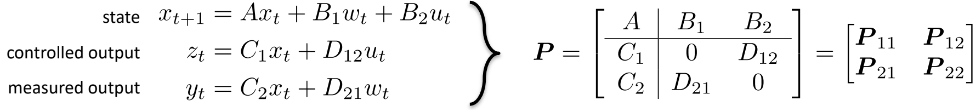
\includegraphics[scale=.45]{figures/plant.png}
        \caption{Generalized plant}
        \label{fig:my_label}
    \end{figure}
This is a generalized state feedback system where $B_1w_t$ is the process disturbance noise and $B_2u_t$ is the input. $z_t$ is the controlled output in which we are trying to keep small, i.e a weighted sum of the deviations from the point of the state that we are trying to maintain. Finally, $y_t$ is the measured output which can be used for the feedback controller. 
P can be looked as a transfer function which maps signals to signals. The map is given by:
\begin{align*}
    \textbf{P}_{ij} = C_i(\hat{z}I-A)^{-1}B_j + D_{ij}
\end{align*}
Now given a feedback controller K:
\begin{figure} [H]
    \centering
    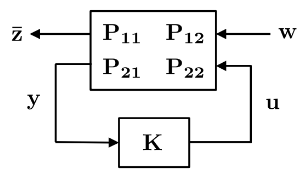
\includegraphics[scale=.4]{figures/feedbackcontroller.png}
    \caption{Feedback Controller}
    \label{fig:feedbackcontroller}
\end{figure}
Where y is the measured output and u the input. We want to find a linear time-invariant controller $u_t = K(y_{0:t})$ that minimizes the "size" of the map from \textbf{w} $\xrightarrow{}$ \textbf{z}. 
Take the $\hat{z}$ transform of our controller such that:
\begin{align*}
    \textbf{u}=\textbf{Ky}
\end{align*}
Where \textbf{bold} font denotes transfer matrices and signals and normal font to denote static matrices and instantaneous values in time. Working in transfer function domain, we take the $\hat{z}$ transform of our dynamics in order to get the mapping \textbf{w} $\xrightarrow{}$ \textbf{z}:
\begin{align*}
    \textbf{x} &= (\hat{z}I-A)^{-1}B_1\textbf{w}+(\hat{z}I-A)^{-1}B_2\textbf{u}\\
    \textbf{z} & = C_1(\hat{z}I-A)^{-1}B_1\textbf{w} + (C_1(\hat{z}I-A)^{-1}B_2 + D_{12u})\textbf{u}\\
    \textbf{z} &= \textbf{P}_{11}\textbf{w}+\textbf{P}_{12}\textbf{u} &&[\text{Substitute in: } \textbf{u}=\textbf{Ky}]\\
    \textbf{z} &= \textbf{P}_{11}\textbf{w}+\textbf{P}_{12}\textbf{Ky} && (1)\\
    \textbf{y} &= C_2(\hat{z}I-A)^{-1}B_1\textbf{w} + C_2(\hat{z}I-A)^{-1}B_2\textbf{u}+D_{21}\textbf{w}\\
    \textbf{y} &= \textbf{P}_{21}\textbf{w}+\textbf{P}_{22}\textbf{u}&&[\text{Substitute in: } \textbf{u}=\textbf{Ky}]\\ 
    \textbf{y} &= \textbf{P}_{21}\textbf{w}+\textbf{P}_{22}\textbf{Ky}  &&(2)\\
    \textbf{y} &= (I-\textbf{P}_{22}K)^{-1}\textbf{P}_{21}w \\
    \textbf{z}&=(\textbf{P}_{11}+\textbf{P}_{12}\textbf{K}(I-\textbf{P}_{22}\textbf{K})^{-1}\textbf{P}_{21})\textbf{w} && (2) \text{ in } (1)\\
    \textbf{z}&=: S(\textbf{P},\textbf{K})\textbf{w}
\end{align*}
The goal is to minimize the mapping from \textbf{w} $\xrightarrow{}$ \textbf{z} which can be given as:\\
\begin{align*}
    \min_{\textbf{K}}\norm{S(\textbf{P},\textbf{K})\textbf{w}}_{norm}
\end{align*}
In the following sections we will look to define different norms that can be used to minimize the linear mapping.
\section{Three Representations of Linear Maps}
\begin{align*}
    \textbf{z}&=(\textbf{P}_{11}+\textbf{P}_{12}\textbf{K}(I-\textbf{P}_{22}\textbf{K})^{-1}\textbf{P}_{21})\textbf{w}\\
    &=: S(\textbf{P},\textbf{K})\textbf{w}
\end{align*}
If we are given \textbf{K} that stabilizes \textbf{P} then S(\textbf{P},\textbf{K}) is a linear map acting on signal \textbf{w}. The goal is minimize the "amplification", "gain", or "size" of map S(\textbf{P},\textbf{K}) taking \textbf{w}$\xrightarrow{}$\textbf{z}.\\

How do we measure the size of S(\textbf{P},\textbf{K}) which we will now call \textbf{M} is determined by how we model disturbance \textbf{w}. We start with analysis, i.e., assume we are given some stable closed loop system \textbf{M} such that:
\begin{center}
\textbf{z} = \textbf{Mw}    
\end{center}
Assuming \textbf{M} is stable, it has a finite gain which does not take a finite \textbf{w} to and infinite \textbf{z}. Let's consider different norms, and their interpretation from a modeling perspective, for measuring "size" of \textbf{M}.\\

There are three representations of these linear maps. Consider a bounded linear-time-invariant operator \textbf{M}: $l^{q}_{\infty} \xrightarrow{} l^p_{\infty}$. q and p are the dimensions of the bounded input, bounded output. We can think of \textbf{M} in three ways:
\begin{enumerate}
    \item As a transfer matrix acting via multiplication: \textbf{z}(z) = \textbf{M}(z)\textbf{w}(z), where \textbf{M}(z) = $\sum^{\infty}_{t=0}\frac{1}{z^t}M_t$ [Power series expansion]
    \item As a linear filter acting via convolution: $z_t = \sum^t_{k=0} M_k w_{t-k}, \forall t \geq 0$. $w_{t-k}$ is the history of disturbance.
    \item As a semi-infinite block Toeplitz matrix mapping signals to signals. Over a finite-time horizon this map should be used with block lower triangular map and the same values along the block diagonals:
    \begin{figure} [H]
        \centering
        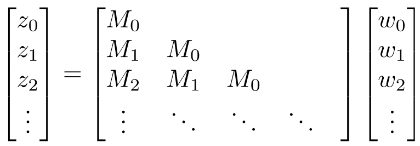
\includegraphics[scale=.5]{figures/toeplitz.png}
        \caption{Semi-infinite block Toeplitz Matrix}
        \label{fig:toeplitz}
    \end{figure}
\end{enumerate}

Let's formalize the operator \textbf{M} in terms of the linear time-invariant systems. In our application, \textbf{M} is called the time-invariant shift operator.\\ 
A shift operator $S_{\tau}:L_2(-\infty,\infty) \xrightarrow{} L_2(-\infty,\infty)$ is defined by:
\begin{align*}
    y = S_{\tau}u \Longleftrightarrow{} y(t) = u(t-\tau)
\end{align*}
\quad This also known as the $\tau$-delay.\\ \\
Definition of time-invariance.\\
An operator $G: L_2(-\infty,\infty) \xrightarrow{} L_2(-\infty,\infty)$ is called time-invariant if:
\begin{align*}
    GS_{\tau} = S_{\tau}G  \qquad \forall \tau \geq 0
\end{align*}
Theorem.\\
An operator $G: L_2(-\infty,\infty) \xrightarrow{} L_2(-\infty,\infty)$ is time-invariant if and only there exists a function  $\hat{G} \in \hat{L}_{\infty}(j \mathbb{R})$ such that the multiplication operator satifies:\\
\begin{align*}
    G = \Phi ^{-1}M_{\hat{G}}\Phi
\end{align*}

\section{System Norms}
Consider a bounded linear time invariant operator \textbf{M}: $l^{q}_{\infty} \xrightarrow{} l^p_{\infty}$ such that \textbf{z} = \textbf{Mw}\\ \\
Theorem [ref: pg20]
The space of all bounded, linear, causal operators from $l_{\infty}^p$ to $l_{\infty}^q$ is given by the space of all infinite block lower triangular matrices, with a finite induced norm, i.e., 
\begin{align*}
    \sup_k\lvert(R_k)\rvert_1 < \infty,\\
\end{align*}
where $(R_k)$ is the $k^{th}$ dimensional block of the matrix R:\\
\begin{align*}
    \begin{bmatrix} R(0,0)&0&\dots&0\\R(1,0)&R(1,1)&0\dots\\ \vdots&\vdots&\vdots&\ddots\\
    R(k,0)&R(k,1)&\dots&R(k,k)\\
    \end{bmatrix}\\
\end{align*}
Equivalently,\\
\begin{align*}
    \sup_i\lvert(R(i,0)) \dots R(i,i)\rvert_1 < \infty
\end{align*}

\begin{enumerate}
    \item Let $w_t$ be \textit{iid} $\mathcal{N}(0,I)$, characterizes average energy amplification from \textbf{w}$\xrightarrow{}\textbf{z}$ as:
    \begin{align*}
       \norm{\textbf{M}}_{H_2}^2 &=\sum^{\infty}_{t=0}\norm{M_T}^2_F\\
       &=\frac{1}{2\pi}\int^{\pi}_{-\pi}\DeclareMathOperator{\Tr}{Tr}M^(e^{jw})M^T(e^{-jw})dw\\
    \end{align*}
    \item For $l_2$-bounded \textbf{w}, worst case energy amplification measured by:
    \begin{align*}
        \norm{\textbf{M}_T}_{H_{\infty}} = \lim_{T\xrightarrow{}\infty}\norm{\Bar{M}_T}_{2\xrightarrow{}2}= \sup_{\omega\in[-\pi,\pi]}\norm{\textbf{M}(e^{jw})}_{2\xrightarrow{}2}
    \end{align*}
    \item For $l_{\infty}$-bounded \textbf{w}, worst case real-time deviations as measured by:
    \begin{align*}
        \norm{\textbf{M}}_{L_1} = \lim_{T\xrightarrow{}\infty}\norm{\bar{M}_T}_{\infty\xrightarrow{}\infty} = \max_{1\leq i\leq p}\sum_{j=1}^q \norm{\textbf{M}^{ij}}_{l_1}
    \end{align*}
\end{enumerate}
Where the $H_{\infty}$ and $L_1$ norms are $l_p \xrightarrow{} l_p$ induced norms.
\subsection{H2 (LQR) Norm}
    Let $w_t$ be \textit{iid} $\mathcal{N}(0,I)$ and \textbf{z} = \textbf{Mw}.  \\
    Looking at \textbf{w}, it is often used to model natural stochastic processes such as thermodynamic noise, aggregate behaviors, etc. The natural notion is to characterize average "energy amplification" of white noise as measured by finite output. Suppose we want to characterize:
    \begin{align*}
        \lim_{T\xrightarrow{}\infty}\frac{1}{T}\sum^T_{t=0}\mathbb{E}\norm{z_t}^2_2
    \end{align*}
    Look at the above as the system's behavior as it goes to some steady state distribution. Therefore, it only depends on its covariance.\\
    For a finite T, $z_t = M_t w_t$
    \begin{align*}
        &= \frac{1}{T}\sum^T_{t=0}\mathbb{E}_w\norm{z_t}^2_2
    \end{align*}
    \begin{center}
        $        z^{(T)} = \begin{bmatrix}z_0\\z_1\\\vdots\\z_T\end{bmatrix}\quad w^{(T)}=\begin{bmatrix}w_0\\w_1\\\vdots\\w_T\end{bmatrix} \quad
        \Bar{M}_T = \begin{bmatrix}M_0\\M_1 & M_0\\ \vdots &\ddots&\ddots\\M_T&\dots&M_1&M_0 \end{bmatrix}$
    \end{center}
    \begin{align*}
        &=\frac{1}{T}\mathbb{E}_w\norm{z^{(T)}}^2_2 && z^{(T)}=\Bar{M}_T w^{(T)}\\
        &=\frac{1}{T}\mathbb{E}_w (w^{(T)})^T \Bar{M}_T^T\Bar{M}_T w^{(T)}\\
        &=\frac{1}{T}\mathbb{E}_w \Bar{M}_T^T\Bar{M}_T w^{(T)}(w^{(T)})^T  &&\text{[cyclic property of trace on $w^{(T)}$]}\\
        &=\frac{1}{T}\DeclareMathOperator{\Tr}{Tr}(\Bar{M}_T^T\Bar{M}_T)\\
        &=\frac{1}{T}\norm{\Bar{M}_T}^2_F\\
        &=\frac{1}{T}(T\norm{M_0}^2_F + (T-1)\norm{M_1}^2_F+\dots+\norm{M_T}^2_F)\\
    \end{align*}
    Take the limit of T $\xrightarrow{} \infty$: 
    \begin{align*}
        =\sum^{\infty}_{t=0}\norm{M_T}^2_F
    \end{align*}
    Use Parseval's Theorem to write the above as an integral over frequency. Which states that the fourier transform does not change the 2 norm.
    \begin{align*}
        &=\frac{1}{2\pi}\int^{\pi}_{-\pi}\DeclareMathOperator{\Tr}{Tr}M^*(e^{jw})M(e^{jw})dw\\
        &:= \norm{M}^2_{H2}
    \end{align*}
    This is known as the H2 norm squared. We are computing the average energy amplification of white noise by the system.\\
    
\subsection{$H_{\infty}$ Norm}
\subsubsection{Finite case}
    Suppose the disturbance process has \textit{bounded finite energy}:
    \begin{align*}
        \norm{\textbf{w}}^2_2 := \sum^{\infty}_{t=0}\norm{w_t}^2_2 < \infty
    \end{align*}
    We can expect signals outputted by stable systems satisfy this property. Used to capture effects of unmodeled dynamics on behavior. Without any spectral or statistical properties, natural notion is to characterize worst-case gain:
    \begin{align*}
        \norm{\textbf{M}}_{H_{\infty}} := \sup_{\norm{\textbf{w}}_2^2\leq1}\norm{\textbf{Mw}}_2^2 && \text{[signal $\xrightarrow{}$ signal, $l_2\xrightarrow{}l_2$, time domain interpretation]}
    \end{align*}
    Find the finite w to max the 2 norm of z. Starting with the finite horizon setting:
    \begin{align*}
        \begin{bmatrix}z_0\\z_1\\\vdots\\z_T\end{bmatrix} =  
        \begin{bmatrix}M_0\\M_1 & M_0\\ \vdots &\ddots&\ddots\\M_T&\dots&M_1&M_0 \end{bmatrix}\begin{bmatrix}w_0\\w_1\\\vdots\\w_T\end{bmatrix} \xrightarrow{} \norm{\textbf{M}_T}_{H_{\infty}} = \norm{\Bar{M}_T}_{2\xrightarrow{}2}
    \end{align*}
    Which can be looked at as the maximum singular value in the finite time horizon. To prove, we have\\
    $z_{(t)} = \Bar{M}_{T}w_{(T)}$
    \begin{align*}
        \norm{\Bar{M}_T}_{2\xrightarrow{}2} &= \sup_{\norm{\textbf{w}}_2^2\leq1}\norm{M_{(T)}w_{(T)}}^2_2\\
        &= \sup_{\norm{\textbf{w}}_2^2\leq1} w_{(T)}^T\Bar{M}_T^T\Bar{M}_T w_{(T)} &  \text{Let } \Bar{M}_T = U\Sigma V^T\\
        &=\sup_{\norm{\textbf{w}}_2^2\leq1}w_{(T)}^T V(\Sigma^T\Sigma)V^T w_{(T)} & \text{Notice} \norm{V^Tw}^2_2 = \norm{w}^2_2 \text{since V is on B}\\
         &=\sup_{\norm{\textbf{w}}_2^2\leq1}w_{(T)}^T (\Sigma^T\Sigma) w_{(T)} & \text{For } \Sigma^T\Sigma = \text{diag}(\sigma_1^2,\sigma_2^2,\dots,\sigma_r^2)\\
         &=\sup_{\norm{\textbf{w}}_2^2\leq1}w_{(T)}^T \text{diag}(\sigma_1^2,\sigma_2^2,\dots,\sigma_r^2) w_{(T)} & (\sigma_1\geq\sigma_2\geq\dots\geq\sigma_r>0)\\
         &= \sigma_1^2
    \end{align*}
    \begin{align*}
        \norm{\textbf{M}_T}_{H_{\infty}} = \norm{\Bar{M}_T}_{2\xrightarrow{}2} = \sigma_1 = \sigma_{max}(M) 
    \end{align*}
%\subsubsection{Infinite Case}

\subsection{$L_1$ Norm}
Suppose the disturbance process has \textit{bounded magnitude}:
    \begin{align*}
        \norm{w}_{l_{\infty}} = \sup_{t\geq0} \norm{w_t}_{\infty} < \infty
    \end{align*}
Consider characterizing the worst-case gain of a system, \textbf{z} = \textbf{Mw} such that:
    \begin{align*}
        \norm{\textbf{M}}_{L_{1}} = \sup_{\norm{w}_{\infty}\leq 1}\norm{\textbf{Mw}}_{\infty} && [\text{signal $\xrightarrow{}$ signal, }l_{\infty}\xrightarrow{}l_{\infty}\text{, time-domain interpretation}]
    \end{align*}
This is useful for real-time safety constraints, i.e. actuator saturation, bumps in a path.\\
\subsubsection{Finite case}
In the finite horizon setting:
    \begin{align*}
        \begin{bmatrix}z_0\\z_1\\\vdots\\z_T\end{bmatrix} =  
        \begin{bmatrix}M_0\\M_1 & M_0\\ \vdots &\ddots&\ddots\\M_T&\dots&M_1&M_0 \end{bmatrix}\begin{bmatrix}w_0\\w_1\\\vdots\\w_T\end{bmatrix} \xrightarrow{} \norm{\textbf{M}_T}_{L_1} = \norm{\Bar{M}_T}_{\infty\xrightarrow{}\infty}
    \end{align*}
    \begin{align*}
        \norm{\Bar{M}_T}_{\infty\xrightarrow{}\infty} &= \sup_{\norm{w^{(T)}}_{\infty}\leq 1}\norm{\bar{M}_T w^{(T)}}_{\infty}\\
        &=\sup_{\norm{w^{(T)}}_{\infty}\leq 1}\norm{\begin{bmatrix}M_0\\M_1 & M_0\\ \vdots &\ddots&\ddots\\M_T&\dots&M_1&M_0\end{bmatrix}
        \begin{bmatrix}w_0\\w_1\\\vdots\\w_T\end{bmatrix}}_{\infty} & \text{Pick the largest row, i.e. the last row}\\
        &=\sup_{\norm{w^{(T)}}_{\infty}\leq 1}\norm{\begin{bmatrix}M_T & M_{T-1}&\dots& M_1& M_0\end{bmatrix}\begin{bmatrix}w_0\\w_1\\\vdots\\w_T\end{bmatrix}}_{\infty} & \text{Where, $z\in \mathbb{R}^p$ and $w\in \mathbb{R}^q$}\\
        &= \max_{1\leq i \leq p}\sum^{(T+1)q}_{j=1}\lvert M^{ij}\rvert\\
        &= \max_{1\leq i \leq p}\sum^T_{t=0}\sum^q_{j=1}\lvert M^{ij}\rvert & \text{Where T is blocks, i rows, j columns}\\
        &= \max_{1\leq i \leq p}\sum^q_{j=1}\sum^T_{t=0}\lvert M^{ij}\rvert\\
        &=\max_{1\leq i\leq p}\sum_{j=1}^q \norm{\textbf{M}^{ij}}_{l_1}\\
    \end{align*}
    Where $M^{ij}$ operator can be defined as:
    \begin{align*}
        M(z) = \begin{bmatrix}M_{11}(z)&M_{12}(z)&\dots&M_{1q}(z)\\ \vdots&\vdots&\ddots&\vdots \\ M_{p1}(z)&\dots&\dots&M_{pq}(z)\end{bmatrix}
    \end{align*}
    $L_1$ can be thought of as taking the max row sum of a matrix.
    
    
%\subsubsection{Infinite case}
%    \begin{align*}
%            &:= \max_{1\leq i\leq p}\sum_{j=1}^q\sum_{t=0}^T \lvert M_t^{ij}\rvert\\
%        &:=\max_{1\leq i\leq p}\sum_{j=1}^q \norm{\textbf{M}^{ij}}_{l_1}\\
%        M_{l_{\infty}\xrightarrow{}l_{\infty}} = \sup_{\norm{w}_{\infty}\leq %1}\norm{\textbf{Mw}}_{\infty}
%    \end{align*}

\section{Modeling Uncertainty}
What if our system M is uncertain? How can you ensure that if my nominal model is stable, bounded, etc., that any possible realization is well-behaved too? First, we need to explicitly model out uncertainty. We are going to focus our analysis on the following interconnection:
\begin{figure} [H]
    \centering
    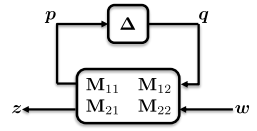
\includegraphics[scale=.7]{figures/deltablock.png}
    \caption{Framework for modeling uncertainty}
    \label{fig:delta}
\end{figure}
for $\Delta \in \textbf{D}$ some set of uncertainty when can we guarantee that this interconnection is stable $\forall \Delta \in \textbf{D}$.\\
Assuming M is stable:
\begin{align*}
    \begin{bmatrix}p\\z\end{bmatrix} = \begin{bmatrix}M_{11} & M_{12}\\M_{21}&M_{22}\end{bmatrix}\begin{bmatrix}q\\w\end{bmatrix} && q = \Delta p
\end{align*}
Solve for $w \xrightarrow{} z$ map: Assume $(I - M_{11}\Delta)^{-1}$ exists for now.
\begin{align*}
    p &= M_{11}q + M_{12}w = M_{11}\Deltap + M_{12}w  \quad \xrightarrow{} \quad p = (I - M_{11}\Delta)^{-1}M_{12}w\\
    z &= M_{21}q + M_{22}w\\
    z &= (M_{22} + M_{21}\Delta(I - M_{11}\Delta)^{-1}M_{12})w\\
    &=: S(M,\Delta)w
\end{align*}
Notice when $\Delta=0$ recovers "nominal" model \textbf{z} = $\textbf{M}_{22}\textbf{w}$. This is a very flexible framework.

\section{Linear Fractional Transform (LFT) Representations of Uncertainty}
For the framework [\ref{fig:delta}], we can pick these $M_{ij}s$ to capture our different types of uncertainties in the following equation:
Assuming $((I - M_{11}\Delta)^{-1})$ exists:
\begin{align*}
        z &= (M_{22} + M_{21}\Delta(I - M_{11}\Delta)^{-1}M_{12})w\\
    &=: S(M,\Delta)w
\end{align*}
So what if we had:
\begin{enumerate}
    \item Additive Uncertainty:
    \begin{align*}
        z = (\hat{G} + \Delta)w \Longleftrightarrow M = \begin{bmatrix}0& I\\I & \hat{G}\end{bmatrix}
    \end{align*}
    Notice that this is always stable if $\hat{G}$ and $\Delta \in \textbf{D}$ are stable ($M_{11} = 0$).
    
    \item Multiplicative uncertainty:
    \begin{align*}
        z = \hat{G}(I + \Delta) \Longleftrightarrow M = \begin{bmatrix}0& I\\\hat{G} & \hat{G}\end{bmatrix}
    \end{align*}
    \item Uncertain state-space matrix:
    \begin{align*}
        x_{t+1} = (\hat{A} + \Delta_A)x_t + w_t \Longleftrightarrow x = \frac{1}{z}(\hat{A} + \Delta_A)x + \frac{1}{z}w && \text{[z-transform]}
    \end{align*}
    \begin{align*}
        \begin{bmatrix}p\\x\end{bmatrix} = \begin{bmatrix}(zI-\hat{A})^{-1}&(zI-\hat{A})^{-1}\\(zI-\hat{A})^{-1}&(zI-\hat{A})^{-1}\end{bmatrix}\begin{bmatrix}q\\w\end{bmatrix}
    \end{align*}
    Notice p = x, and q = $\Delta_A x$
    \begin{align*}
        x &= [(zI-\hat{A})^{-1} + (zI-\hat{A})^{-1}\Delta_A(I - (zI-\hat{A})^{-1} \Delta_A)^{-1}(zI-\hat{A})^{-1}]w\\
        &= (zI-\hat{A} - \Delta_A)^{-1}w \qquad \qquad \qquad \qquad \qquad \text{[Woodbury Matrix Identity (Matrix Inversion)]}
    \end{align*}
    Where it is assumed that $(I - (zI-\hat{A})^{-1}\Delta_A)^{-1}$ and $(zI-\hat{A} - \Delta_A)^{-1}$ exist as maps. This property is useful for multiple feedback loops and deals with the nominal framework. Finally, this illustrates that $ x_{t+1} = (\hat{A} + \Delta_A)x_t + w_t$ is stable iff, $(zI-\hat{A})^{-1}$ is stable and $(I - (zI-\hat{A})^{-1}\Delta_A)^{-1}$ is stable.
\end{enumerate}

\section{Robust well-connectedness, Robust Stability, Robust Performance}
We have reduced our analysis to determining the stability of a nominal system interconnected with an uncertain element. Here we show necessary and sufficient conditions where $\Delta \in \textbf{D} \Longleftrightarrow \norm{\Delta}\leq 1$ for an induced norm.

\begin{figure} [H]
    \centering
    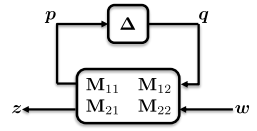
\includegraphics[scale=.7]{figures/deltablock.png}
    \caption{Framework for modeling uncertainty}
    \label{fig:delta}
\end{figure}

Assuming $((I - M_{11}\Delta)^{-1})$ exists:
\begin{align*}
        z &= (M_{22} + M_{21}\Delta(I - M_{11}\Delta)^{-1}M_{12})w\\
    &=: S(M,\Delta)w
\end{align*}
\begin{enumerate}
    \item \textbf{Robust well-connectedness}:\\
    The interconnection illustrated in figure [\ref{fig:delta}] is robustly well-connected if $(I - \textbf{M}_{11}\Delta)^{-1}$ exists for all $\Delta \in \textbf{D}$. If (\textbf{M,D}) is robustly well-connected, then the map $S(M,\Delta)w$ is stable and bounded.
    \item \textbf{Robust stability}:\\
    Ensuring that (\textbf{M},\textbf{D}) is robustly well-connected, i.e., that  $(I - \textbf{M}_{11}\Delta)^{-1}$ exists for all $\Delta \in \textbf{D}$
    \item \textbf{Robust performance}:\\
    Ensuring robust stability and $\norm{S(\textbf{M}, \Delta)} < \gamma \forall \Delta \in \textbf{D}$
\end{enumerate}


\section{Induced Norms}
The $H_{\infty}$ and $L_1$ norms defined previously are both $l_p \xrightarrow{} l_p$ induced norms which can be written as :
\begin{align*}
    \norm{\textbf{M}} = \sup_{\norm{\textbf{w}}\leq 1} \norm{\textbf{Mw}}
\end{align*}
All induced norms satisfy a sub-multiplicative property:
\begin{align*}
    \norm{\textbf{AB}} \leq \norm{\textbf{A}} \cdot \norm{\textbf{B}}
\end{align*}
Which can be thought of as "the gain of two systems is no larger than the product of the individual gains". This property lets us compose maps (systems) through multiplication and remain bounded: allows us to conclude that the set of bounded maps define a Banach Algebra.

\section{Banach Algebra}
Banach algebras allows us to take limits and products without worrying about things being badly behaved. This will be very important for robustness analysis. To define Banach algebras let's look at operators and then the sets of linear operators.\\ \\
For Banach spaces $\mathcal{V}$ and $\mathcal{Z}$, the map F: $\mathcal{V}\xrightarrow{}\mathcal{Z}$ is a bounded linear operator if:
\begin{itemize}
    \item \textit{Linearity}: $F(\alpha_1 v_1 + \alpha_2 v_2) = \alpha_1F(v_1) + \alpha_2 F(v_2)$ for all $v_1,v_2 \in \mathcal{V}$ and $\alpha_1, \alpha_2 \in \mathbb{R}$
    \item \textit{Boundedness}: There exists K > 0 such that $\norm{F(v)} \leq K\norm{v}$ for all $v \in \mathcal{V}$
\end{itemize}
Sets of Linear Operators
\begin{itemize}
    \item     $\mathcal{L}(\mathcal{V,Z})$ is the set of all bounded linear operators mapping $\mathcal{V}$ to $\mathcal{Z}$
    \item   $\mathcal{L(V)}$ is the set of all bounded linear operators mapping $\mathcal{V}$ to itself.
\end{itemize}
The set $\mathcal{L}(\mathcal{V,Z})$ is a Banach space.
\begin{itemize}
    \item It is a vector space; we have addition and scalar multiplication. e.g.
    \begin{align*}
        (F_1 + F_2)(v) = F_1(v) + F_2(v)
    \end{align*}
    \item It has a norm- the induced norm.
    \item It is complete.
\end{itemize}
Therefore, Banach algebras as well as being a normed vector space, the set $\mathcal{L(V)}$ has additional structure, since one map compose maps. We write $(F_1 F_2)(v) = F_1(F_2(v))$, giving:
\begin{align*}
    F_1, F_2 \in \mathcal{L(V)} \quad \Longrightarrow \quad F_1 F_2 \in \mathcal{L(V)}
\end{align*}
Where the space $\mathcal{L(V)}$ is called a Banach algebra. We can use Banach algebra to define small-gain theorem.

\section{Small-Gain Theorem}
Suppose Q is an element of Banach algebra $\mathcal{B}$ i.e. bounded and a linear operator, and \textbf{D}:=\{$\Delta: \norm{\Delta}_{H_{\infty}}\leq 1\}$  then:
\begin{align*}
    \norm{Q} < 1 \quad \Longrightarrow \quad I-Q\Delta \text{ is invertible, and } (I-Q\Delta)^{-1} = \sum_{i=0}^{\infty} (Q\Delta)^i
\end{align*}
Note:
\begin{itemize}
    \item Here we are assuming Q is an element of a Banach algebra. We do not need to use any properties of Q as a linear map.
    \item The submultiplicative property implies $\norm{PQ} \leq \norm{P}\norm{Q}$. Hence if $\norm{P} \leq 1,$ \quad $I-PQ$ is invertible for all operators Q with $\norm{Q} < 1$
\end{itemize}
Proof:\\
\textbf{IF}: $\norm{Q}<1 \quad \Longrightarrow \quad \norm{Q\Delta} \leq \norm{Q}\cdot\norm{\Delta}<1$
\begin{align*}
    (I - Q\Delta)^{-1} &= \sum^{\infty}_{i=0}(Q\Delta)^i &&\text{Limit exists because Banach algebra}\\
    \norm{I-Q\Delta}^{-1} &\leq \sum^{\infty}_{i=0}(\norm{Q}\norm{\Delta})^i< \infty && \text{Since} \norm{Q}\cdot\norm{\Delta}<1
\end{align*}
\textbf{Only IF}: Assume $\norm{Q}_{H_{\infty}^2} = \norm{Q^*}_{H_{\infty}^2} = \lambda_{max}(QQ^*)\geq 1$\\
\begin{align*}
    &\text{Set }\lambda - \lambda_{max}(QQ^*)\geq 1\\
    &\text{Then, }\lambda I - Q Q^* \text{ is singular if }\lambda = \norm{Q^*}_{h_{\infty}}^2 \text{by definition of an eigenvalue.}\\
    &\Longrightarrow I-\frac{QQ^*}{\norm{Q^*}^2_{H_{\infty}}} \text{is singular (multiplication by constant only scalar eigenvalues).}\\
    &\text{Set, } \Delta = \frac{Q^*}{\norm{Q^*}^2_{H_{\infty}}}\quad \Longrightarrow \quad  \norm{\Delta}_{h_{\infty}} = \frac{1}{\norm{Q^*}_{H_{\infty}}} \leq 1 \quad \text{since,} \norm{Q^*}_{H_{\infty}} \geq 1
\end{align*}
Note: $\norm{\Delta}\leq \beta$ needs $\norm{Q}< \frac{1}{\beta}$, (so $\norm{Q\Delta}<1$)

\section{Connection to $H_{\infty}$ Optimal Control}
\begin{figure} [H]
    \centering
    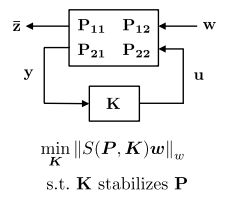
\includegraphics[scale =.7]{figures/optcontrol.png}
    \caption{Framework of Optimal Control}
    \label{fig:optcontrol}
\end{figure}
\begin{align*}
    z &= (P_{11} + P_{12}K( I - P_{22}K)^{-1}P_{21})w\\
    &=: S(P,K)w
\end{align*}

Suppose I compute K s.t. $\norm{S(P_o, K)}_{H_{\infty}} < \frac{1}{\gamma}$\\
Robust stability interpretation: Set $M_{11} = S(P, K)$, then this says,
\begin{figure}[H]
    \centering
    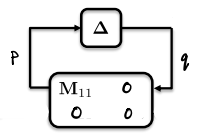
\includegraphics[scale =.7]{figures/robuststability.png}
    \caption{Robust Stability}
    \label{fig:robuststability}
\end{figure}
is robustly well-connected $\forall \Delta$ s.t. $\norm{\Delta}_{H_{\infty}} \leq \gamma$

\section{Equivalence between Robust Performance and Robust Stability}
Robust Performance and Robust Stability are equivalent on an augmented Delta block with respect to two block uncertainty.
\begin{figure} [H]
    \centering
    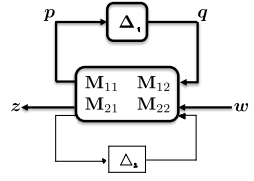
\includegraphics[scale = .7]{figures/augdelta.png}
    \caption{Augmented Delta Block Plant}
    \label{fig:my_label}
\end{figure}
Theorem (the following are equivalent):\\
\begin{itemize}
    \item $(I - \textbf{M}_{11}\Delta_1)^{-1}$ exists and is bounded and $\norm{S(\textbf{M},\Delta_1)}_{H_{\infty}} < 1$ for all $\norm{\Delta_1}_{H_{\infty}}\leq 1$
    \item $(I - \textbf{M}\Delta)^{-1}$ is robustly well connected for all $\Delta = \begin{bmatrix}\Delta_1& \\&\Delta_2\end{bmatrix}$, $\norm{\Delta_1}_{H_{\infty}}, \norm{\Delta_2}_{H_{\infty}} \leq 1$
\end{itemize}
Proof: (1 $\xrightarrow{}$ 2):\\
\begin{align*}
    I- \begin{bmatrix}M_{11}&M_{12}\\M_{21}&M_{22}\end{bmatrix}\begin{bmatrix}\Delta_1& \\&\Delta_2\end{bmatrix} &= \begin{bmatrix}I-M_{11}\Delta_1 & -M_{12}\Delta_2 \\ -M_{21}\Delta_2 & I-M_{22}\Delta_2 \end{bmatrix}\\
    &= \begin{bmatrix}I&\\ -M_{21}\Delta_1&I \end{bmatrix}\begin{bmatrix}I-M_{11}\Delta_1 & -M_{12}\Delta_2 \\ 0 & I-M_{22}\Delta_2 \end{bmatrix}
\end{align*}
So if $I- M\Delta$ is invertible iff $I-S(M,\Delta_1)\Delta_2$ is invertible for all $\norm{\Delta_2}\leq 1$, but we know by assumption that $\norm{S(M,\Delta_1)}<1$\\ \\
(2 $\xrightarrow{}$ 1):\\
So by assumption $I- M\Delta$ is invertible for all $\begin{bmatrix}\Delta_1& \\&\Delta_2\end{bmatrix}, \norm{\Delta_1}_{H_{\infty}}, \norm{\Delta_2}_{H_{\infty}} \leq 1$\\
Pick $\begin{bmatrix}\Delta_1& \\&0\end{bmatrix}$ $\Longrightarrow$ $I- M_{11\Delta_1}$ is invertibl for all $\norm{\Delta_1}\leq 1$\\
Then you can write:\\
$I- M\Delta = \begin{bmatrix}I&\\ -M_{21}\Delta_1&I \end{bmatrix}\begin{bmatrix}I-M_{11}\Delta_1 & -M_{12}\Delta_2 \\ 0 & I-M_{22}\Delta_2 \end{bmatrix}$ (Since $(I- M_{11}\Delta)^{-1}$ exists) to conclude using small gain theorem that $\norm{S(M,\Delta_1)}<1 $ for all $\norm{\Delta} \leq 1$

\section{Analysis of Two-Cart and Spring System}
Given \cite{MatlabRobust} the following system of two frictionless carts connected by spring k with uncertain elements, let's analyze the robustness of the feedback control system by evaluating the worst case gain of this uncertain state-space model.
\begin{figure} [H]
    \centering
    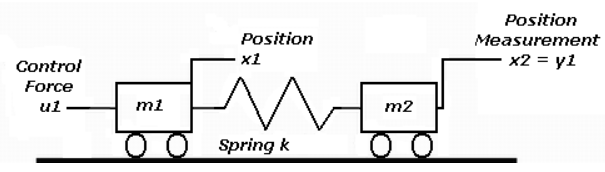
\includegraphics[scale=.5]{figures/2cart.png}
    \caption{Two-cart and spring system}
    \label{fig:2cart}
\end{figure}
\begin{figure} [H]
    \centering
    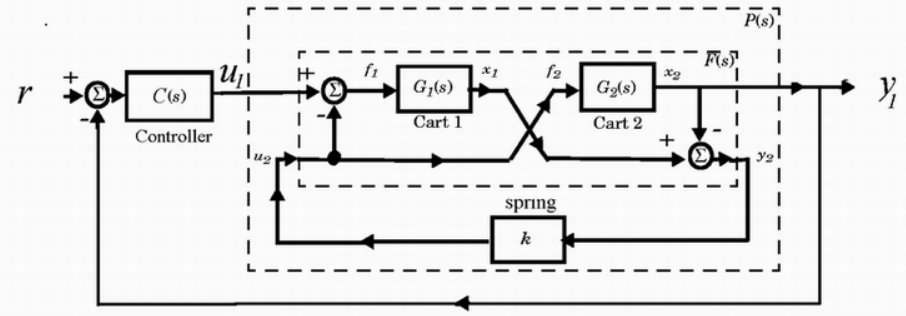
\includegraphics[scale=.3]{figures/block2cart.png}
    \caption{Block diagram of two-cart and spring system}
    \label{fig:block2cart}
\end{figure}

The feedback control is given by $u_1 = C(s)(r-y_1)$ with an input force force $u_1$ and the output being the position $y_1$. The triple-lead compensator is given by $C(s) = \frac{100(s+1)^3}{(0.001s + 1)^3}$.\\
The difficulty in controlling this system is the fact that some of the parameters are uncertain to a degree. The values of the spring constant k and cart masses $m_1, m_2$ are known with only an accuracy of 20\%.
\begin{align*}
    k = 1.0 \pm 20\%\\
    m_1 = 1.0 \pm 20\%\\
    m_2 = 1.0 \pm 20\%\\
\end{align*}
In Matlab, the ureal function can be used to create these three uncertain real parameters. Now, let's construct the uncertain state-space models for the $G_1$ and $G_2$:
\begin{align*}
    G_1 = \frac{1}{m_1 s^2}
    G_2 = \frac{1}{m_2 s^2}
\end{align*}
Looking at the block diagram [\ref{fig:block2cart}], construct the closed loop transfer function.
\begin{align*}
    F &= [0;G1]*[1 -1]+[1;-1]*[0,G2] & \text{Spring-less inner block F(s)}\\
    P &= \text{lft}(F,k) &\text{Connect with spring k}\\
    L &= P*C & \text{Uncertain open-loop model}\\
    T &= \text{feedback}(L,1) & \text{Uncertain closed-loop model}
\end{align*}
T is a uncertain continuous-time state-space model with 1 outputs, 1 inputs, 7 states. The model uncertainty lies in blocks: k, $m_1$, $m_2$. The nominal system can be checked to see if it has negative real parts.\\
\begin{align*}
    \text{maxrealpole} = -0.8232
\end{align*}
We can find the robust stability margin of the system, i.e. will the feedback loop remain stable for all possible values of k, $m_1$, $m_2$ in the specified uncertainty range?\\
Matlab's output using robstab to analyze:\\
Computing peak...  Percent completed: 100/100\\
System is robustly stable for the modeled uncertainty.\\
 -- It can tolerate up to 288\% of the modeled uncertainty.\\
 -- There is a destabilizing perturbation amounting to 289\% of the modeled uncertainty.\\
 -- This perturbation causes an instability at the frequency 575 rad/seconds.\\
 -- Sensitivity with respect to each uncertain element is:           \\
      12\% for k. Increasing k by 25\% decreases the margin by 3\%.    \\
      47\% for m1. Increasing m1 by 25\% decreases the margin by 11.8\%.\\
      47\% for m2. Increasing m2 by 25\% decreases the margin by 11.8\%.\\ \\
Worst case (wcu), the smallest destabilizing parameter relative to nominal values:\\
k: 1.5773\\
m1: 0.4227\\
m2: 0.4227\\

These values can be interpreted as the closed loop can tolerate up to almost three times as much variability in the uncertain elements before going unstable. The smallest destabilizing value for each of the uncertain parameters is also given above.\\ \\
The worst case gain across frequency of the closed loop T can be found with wcgain.
\begin{align*}
    \text{PeakGain} =& \\
           &\text{LowerBound}: 1.0471\\
           &\text{UpperBound}: 1.0797\\
    &\text{CriticalFrequency}: 7.7644\\
\end{align*}

With the wcu computed before, we can compute the worst-case closed-loop transfer Twc. We can now pick random samples of uncertain parameters in the nominal T and compare it with the Twc.
\begin{figure} [H]
    \centering
    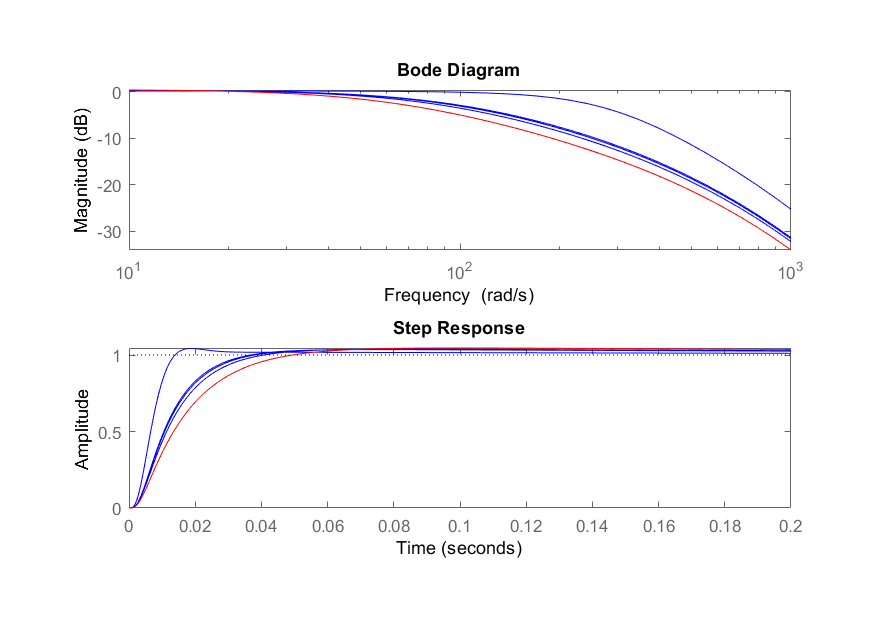
\includegraphics[scale =.6]{figures/Twc.png}
    \caption{T (nominal, blue) vs Twc (worst case, red)}
    \label{fig:my_label}
\end{figure}

Finally, we can examine the worst-case frequency response using wcsigma.
\begin{figure}[H]
    \centering
    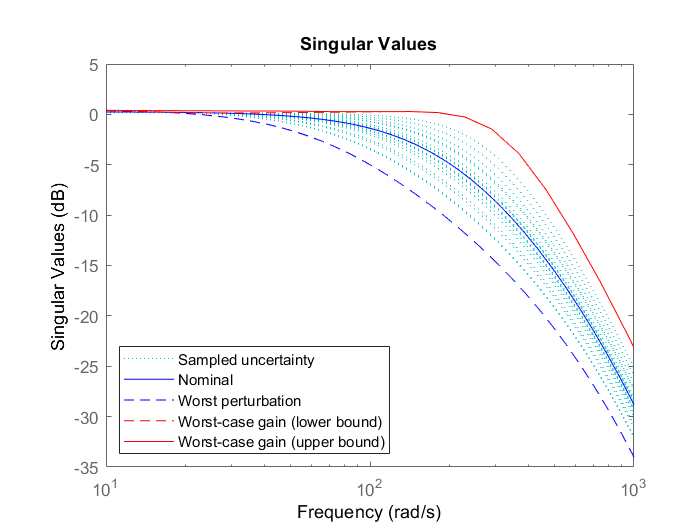
\includegraphics[scale=.6]{figures/wcsigma.png}
    \caption{Worst-case frequency response}
    \label{fig:wcgain}
\end{figure}
\clearpage
\bibliographystyle{abbrvnat}
\bibliography{references}

\begin{thebibliography}{5}
\bibitem{Norms}
\textit{Norms for Signals and Systems}
\url{http://www.cds.caltech.edu/~macmardg/courses/cds110b/dft/dft92-ch2.pdf}

\bibitem{Linear Analysis}
S. Lall.
\textit{Engr210a Lecture 6: Linear analysis and systems}
\url{http://floatium.stanford.edu/engr210a/lectures/ $lecture6\_2001\_10\_\17\_01$.pdf}.
2001.

\bibitem{LFTs}
S. Lall.
\textit{Engr210a Lecture 17: LFTs and robustness}
\url{http://floatium.stanford.edu/engr210a/lectures/ $lecture17\_2001\_12\_03\_02$.pdf}.
2001.

\bibitem{Control of Uncertain}
M.A. Dahleh, I.J. Diaz-Bobillo.
\textit{Control of Uncertain Systems.}
1995.

\bibitem{MatlabRobust}
\textit{Building and Manipulating Uncertain Models.}
\url{https://www.mathworks.com/help/robust/examples/building-and-manipulating-uncertain-models.html}.
Matlab, Robust Control Toolbox.


\end{thebibliography}
%
 \end{document}






